\chapter{रसायनज्ञों के लिए क्वांटम यांत्रिकी: मॉडल निकाय}\label{ch:b3:quantum-model-systems}

एक बेंच पर तीन छोटे फ़्लास्क रखे हैं, और हर एक में एथेनॉल में घुले किसी सायनिन
रंजक का विलयन है: पहला मैजेंटा है, दूसरा नीला, तीसरा गहरा हरिताभ नीला जो सुदूर
लाल में अवशोषण करता है। तीनों अणु एक ही ढंग से बने हैं --- नाइट्रोजन युक्त दो
सर्वसम वलय, जिन्हें कार्बन परमाणुओं की एक शृंखला जोड़ती है --- और वे केवल उस
शृंखला की लंबाई में भिन्न हैं, हर बार दो कार्बन परमाणुओं के अंतर से। शृंखला
लंबी कीजिए और रंग लाल की ओर खिसक जाता है। 1949 के एक रसायनज्ञ ने इस श्रेणी की
व्याख्या क्वांटम यांत्रिकी की सबसे सरल समस्याओं में से एक से की: नियत लंबाई की
रेखा पर गति करने को स्वतंत्र एक इलेक्ट्रॉन, ``\omterm{def:b3:quantum-model-systems:box}{डिब्बे में कण}''। यह अध्याय उस
व्याख्या के पीछे का तंत्र खड़ा करता है --- \omterm{def:b3:quantum-model-systems:operator}{संकारक}, \omterm{def:b3:quantum-model-systems:operator}{अभिलक्षणिक मान}, \omterm{thm:b3:quantum-model-systems:schrodinger}{श्रोडिंगर
समीकरण} --- और उन मॉडल निकायों को हल करता है जिनका उपयोग रसायन विज्ञान प्रतिदिन
करता है: डिब्बा, कंपन करते आबंध का \omterm{def:b3:quantum-model-systems:oscillator}{आवर्ती दोलित्र}, घूमते अणु का \omterm{def:b3:quantum-model-systems:rotor}{दृढ़ घूर्णक},
हाइड्रोजन परमाणु, और वह अवरोध जिसे कोई हल्का कण उस पर चढ़ने की ऊर्जा के बिना
भी पार कर सकता है।

\begin{recall}
प्रथम वर्ष के खंड ने दिखाया था कि परमाणु की ऊर्जा क्वांटीकृत है (ऊर्जा स्तर,
मूल और उत्तेजित अवस्थाएँ, हाइड्रोजन की रेखाएँ) और कि एक फ़ोटॉन
$E = h\nu = hc/\lambda$ ऊर्जा वहन करता है। द्वितीय वर्ष के खंड ने इलेक्ट्रॉन का वर्णन
एक तरंग फलन $\psi$ से किया जिसका वर्ग प्रायिकता घनत्व है, हाइड्रोजन के कक्षकों को
त्रिज्य और कोणीय भागों में बाँटा, और उनके नोड गिने; हाइड्रोजन के तरंग फलनों को
उसने दिया हुआ माना था। यहाँ, अनुभाग 5 में, वे व्युत्पन्न किए गए हैं। भौतिकी से:
संवेग $p = mv$ और दे ब्रॉग्ली तरंगदैर्घ्य
$\lambda = h/p$।
\end{recall}

\begin{omfigure}
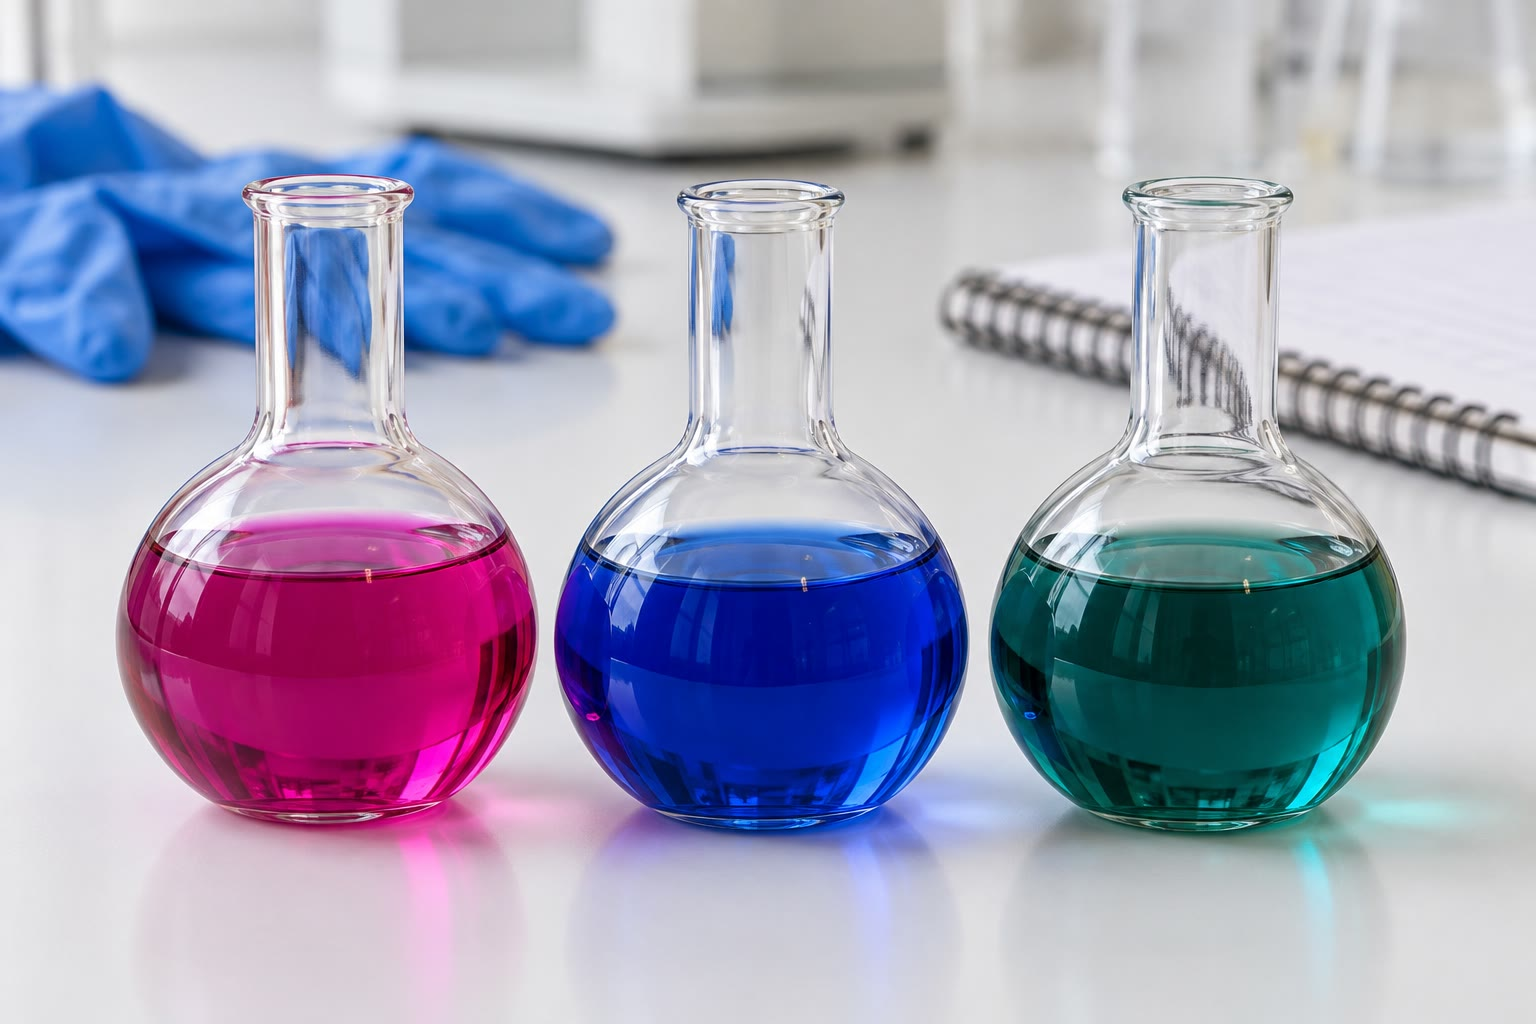
\includegraphics[width=0.62\linewidth]{images/book4/ai/b3-01-dyes.jpg}

{\small एक ही कुल के तीन सायनिन रंजकों के विलयन। शृंखला में जुड़ा कार्बन
परमाणुओं का हर नया युग्म अवशोषण को लाल की ओर खिसका देता है।}
\end{omfigure}

\section{संकारक, अभिलक्षणिक मान और श्रोडिंगर समीकरण}

चिरसम्मत यांत्रिकी किसी कण को हर क्षण एक स्थिति और एक संवेग देती है। क्वांटम
यांत्रिकी उसे एक अवस्था देती है, तरंग फलन $\psi$, और हर मापनीय राशि को
$\psi$ पर की जाने वाली एक संक्रिया से प्रतिस्थापित करती है।

\begin{definition}[संकारक, अभिलक्षणिक फलन, अभिलक्षणिक मान]\label{def:b3:quantum-model-systems:operator}
\emph{संकारक}\index{संकारक} $\hat A$ एक नियम है जो किसी फलन को दूसरे फलन में
बदल देता है: $\hat A f = g$। वह रैखिक है यदि $\hat A(\lambda f +
\mu g) = \lambda\hat Af + \mu\hat Ag$। कोई शून्येतर फलन $f$, जिसके लिए
$\hat Af = a f$ हो, जहाँ $a$ कोई संख्या है, \emph{अभिलक्षणिक फलन}\index{अभिलक्षणिक फलन}
कहलाता है (संकारक $\hat A$ का), और $a$ संगत \emph{अभिलक्षणिक मान}\index{अभिलक्षणिक मान} है।
\end{definition}

\begin{example}[स्थिति और संवेग के दो संकारक]\label{ex:b3:quantum-model-systems:xp}
एक विमा में स्थिति \omterm{def:b3:quantum-model-systems:operator}{संकारक} $x$ से गुणा करता है, $\hat x f = xf$,
और संवेग \omterm{def:b3:quantum-model-systems:operator}{संकारक} अवकलन करता है, $\hat p f = -\iu\hbar\,
\dd f/\dd x$, जहाँ $\hbar = h/2\pi$। फलन $\eu^{\iu kx}$
\omterm{def:b3:quantum-model-systems:operator}{संकारक} $\hat p$ का \omterm{def:b3:quantum-model-systems:operator}{अभिलक्षणिक फलन} है, \omterm{def:b3:quantum-model-systems:operator}{अभिलक्षणिक मान} $\hbar k$ के साथ: तरंगदैर्घ्य
$\lambda = 2\pi/k$ वाली तरंग का संवेग $h/\lambda$ है, यही दे ब्रॉग्ली संबंध है।
फलन $\sin kx$ \omterm{def:b3:quantum-model-systems:operator}{संकारक} $\hat p$ का \omterm{def:b3:quantum-model-systems:operator}{अभिलक्षणिक फलन} नहीं है (उसका अवकलज
कोज्या है), परंतु वह $\hat p^2 = -\hbar^2\,\dd^2/\dd x^2$ का \omterm{def:b3:quantum-model-systems:operator}{अभिलक्षणिक फलन} है,
\omterm{def:b3:quantum-model-systems:operator}{अभिलक्षणिक मान} $\hbar^2k^2$ के साथ।
\end{example}

\begin{definition}[हर्मिटी संकारक, प्रत्याशा मान]\label{def:b3:quantum-model-systems:hermitian}
ऐसे दो फलनों के लिए जो क्षेत्र की परिसीमाओं पर लुप्त होते हैं, $\langle f|g\rangle = \int f^*g\,\dd\tau$
लिखिए। कोई \omterm{def:b3:quantum-model-systems:operator}{संकारक} \emph{हर्मिटी}\index{हर्मिटी संकारक} है
यदि $\langle f|\hat Ag\rangle = \langle \hat Af|g\rangle$, ऐसे सभी
$f$ और $g$ के लिए।
किसी प्रसामान्यीकृत अवस्था $\psi$ ($\langle\psi|\psi\rangle = 1$) में
$\hat A$ का \emph{प्रत्याशा मान}\index{प्रत्याशा मान}
$\langle A\rangle = \langle\psi|\hat A\psi\rangle$ है: सर्वसम रूप से तैयार किए गए
निकायों पर किए गए अनेक मापनों का माध्य।
\end{definition}

क्वांटम रसायन के कार्यकारी नियम --- उसके अभिगृहीत --- अब एक साँस में कहे जा
सकते हैं: हर मापनीय राशि एक \omterm{def:b3:quantum-model-systems:hermitian}{हर्मिटी संकारक} द्वारा निरूपित होती है; कोई मापन
उसके \omterm{def:b3:quantum-model-systems:operator}{अभिलक्षणिक मानों} में से एक देता है; और यदि
$\psi$ \omterm{def:b3:quantum-model-systems:operator}{संकारक} $\hat A$ का \omterm{def:b3:quantum-model-systems:operator}{अभिलक्षणिक फलन} है, तो उस पर किया गया हर मापन वही
मान देता है, उसका \omterm{def:b3:quantum-model-systems:operator}{अभिलक्षणिक मान}।

\begin{theorem}[हर्मिटी संकारक]\label{thm:b3:quantum-model-systems:hermitian-real}
\omterm{def:b3:quantum-model-systems:hermitian}{हर्मिटी संकारक} के \omterm{def:b3:quantum-model-systems:operator}{अभिलक्षणिक मान} वास्तविक होते हैं। भिन्न \omterm{def:b3:quantum-model-systems:operator}{अभिलक्षणिक मानों} वाले दो
\omterm{def:b3:quantum-model-systems:operator}{अभिलक्षणिक फलन} लांबिक होते हैं: $\langle f_1|f_2\rangle = 0$।
\end{theorem}

\begin{proof}
मान लीजिए $\hat Af = af$। तब $\langle f|\hat Af\rangle = a\langle f|f\rangle$ और
$\langle\hat Af|f\rangle = a^*\langle f|f\rangle$। \omterm{def:b3:quantum-model-systems:operator}{संकारक} \omterm{def:b3:quantum-model-systems:hermitian}{हर्मिटी} है,
अतः दोनों बराबर हैं, और $\langle f|f\rangle > 0$: $a = a^*$। अब मान लीजिए $\hat Af_1
= a_1f_1$ और $\hat Af_2 = a_2f_2$, जहाँ $a_1 \ne a_2$, दोनों वास्तविक। तब
$\langle f_1|\hat Af_2\rangle = a_2\langle f_1|f_2\rangle$ और $\langle\hat Af_1|
f_2\rangle = a_1\langle f_1|f_2\rangle$; इनकी समता से $(a_2 - a_1)
\langle f_1|f_2\rangle = 0$ मिलता है, अतः $\langle f_1|f_2\rangle = 0$।
\end{proof}

मापा गया मान एक वास्तविक संख्या होता है, इसीलिए प्रेक्षणीय राशियों का \omterm{def:b3:quantum-model-systems:hermitian}{हर्मिटी}
होना आवश्यक है; लांबिकता ही किसी परमाणु के कक्षकों, या किसी डिब्बे के स्तरों, को
स्वतंत्र अवस्थाओं का एक साफ़ समुच्चय बनाती है।

\begin{definition}[क्रमविनिमेयक]\label{def:b3:quantum-model-systems:commutator}
दो \omterm{def:b3:quantum-model-systems:operator}{संकारकों} का \emph{क्रमविनिमेयक}\index{क्रमविनिमेयक} $[\hat A,\hat B] =
\hat A\hat B - \hat B\hat A$ है। \omterm{def:b3:quantum-model-systems:operator}{संकारक} क्रमविनिमेय होते हैं यदि उनका क्रमविनिमेयक
शून्य हो।
\end{definition}

\begin{example}[विहित क्रमविनिमेयक]\label{ex:b3:quantum-model-systems:canonical}
किसी भी फलन $f$ के लिए, $\hat x\hat pf = -\iu\hbar xf'$ और $\hat p\hat xf =
-\iu\hbar(f + xf')$। अंतर $[\hat x,\hat p]f = \iu\hbar f$ है, अतः
$[\hat x,\hat p] = \iu\hbar$: स्थिति और संवेग क्रमविनिमेय नहीं हैं। यही
एक संबंध अनिश्चितता सिद्धांत का आधार है और, आगे चलकर, \omterm{def:b3:quantum-model-systems:oscillator}{आवर्ती दोलित्र} के पूरे
स्पेक्ट्रम का भी।
\end{example}

\begin{proposition}[क्रमविनिमेय संकारक]\label{prop:b3:quantum-model-systems:commuting}
यदि $\hat A$ और $\hat B$ क्रमविनिमेय हैं और $f$ \omterm{def:b3:quantum-model-systems:operator}{संकारक} $\hat A$ का \omterm{def:b3:quantum-model-systems:operator}{अभिलक्षणिक फलन} है,
जिसका \omterm{def:b3:quantum-model-systems:operator}{अभिलक्षणिक मान} $a$ अनपभ्रष्ट है, तो $f$
\omterm{def:b3:quantum-model-systems:operator}{संकारक} $\hat B$ का भी \omterm{def:b3:quantum-model-systems:operator}{अभिलक्षणिक फलन} है।
\end{proposition}

\begin{proof}
$\hat A(\hat Bf) = \hat B\hat Af = a(\hat Bf)$: फलन $\hat Bf$ या तो
$\hat A$ का \omterm{def:b3:quantum-model-systems:operator}{अभिलक्षणिक फलन} है, उसी \omterm{def:b3:quantum-model-systems:operator}{अभिलक्षणिक मान} $a$ के साथ, या शून्य है।
\omterm{def:b3:quantum-model-systems:operator}{अभिलक्षणिक मान} अनपभ्रष्ट होने से $\hat Bf$, $f$ का एक गुणज है, मान लीजिए $bf$।
\end{proof}

ऊर्जा का \omterm{def:b3:quantum-model-systems:operator}{संकारक} \omterm{def:b3:quantum-model-systems:schrodinger}{हैमिल्टनी संकारक} है। द्रव्यमान $m$ वाले कण के लिए, जो विभव
$V$ में है, चिरसम्मत ऊर्जा $p^2/2m + V$ एक \omterm{def:b3:quantum-model-systems:operator}{संकारक} बन जाती है।

\begin{definition}[हैमिल्टनी संकारक]\label{def:b3:quantum-model-systems:schrodinger}
द्रव्यमान $m$ वाले और विभव $V(\mathbf r)$ में गतिमान कण का
\emph{हैमिल्टनी संकारक}\index{हैमिल्टनी संकारक} यह है:
\[
\hat H = -\frac{\hbar^2}{2m}\nabla^2 + V(\mathbf r), \qquad \nabla^2 =
\frac{\partial^2}{\partial x^2} + \frac{\partial^2}{\partial y^2} +
\frac{\partial^2}{\partial z^2},
\]
और अनेक कणों के लिए, उनके गतिज पदों और उनकी सभी स्थितिज ऊर्जाओं का
योग।
\end{definition}

\begin{theorem}[श्रोडिंगर समीकरण]\label{thm:b3:quantum-model-systems:schrodinger}
किसी निकाय की निश्चित ऊर्जा वाली अवस्थाएँ --- उसकी स्थिर अवस्थाएँ --- उसके
\omterm{def:b3:quantum-model-systems:schrodinger}{हैमिल्टनी संकारक} के \omterm{def:b3:quantum-model-systems:operator}{अभिलक्षणिक फलन} हैं, और उसकी अनुमत ऊर्जाएँ उसके \omterm{def:b3:quantum-model-systems:operator}{अभिलक्षणिक
मान} हैं:
\[
\hat H\psi = E\psi,
\]
यह काल-निरपेक्ष \emph{श्रोडिंगर समीकरण}\index{श्रोडिंगर समीकरण} है।
स्वीकार्य $\psi$ एकमानी, संतत और
वर्ग-समाकलनीय होता है (उसे प्रसामान्यीकृत किया जा सकता है)।
\end{theorem}
\begin{proof}[स्थिति]
यह एक अभिगृहीत है, जिसका औचित्य उसके परिणाम हैं: आगे हल किए गए हर निकाय के
स्तर स्पेक्ट्रमिकी से मेल खाते हैं। काल-आश्रित समीकरण, जिसकी यह स्थिर
स्थिति है, भौतिकी का विषय है।
\end{proof}

क्वांटीकरण परिसीमा प्रतिबंध करते हैं: किसी अवकल समीकरण के हल हर
$E$ के लिए होते हैं, परंतु उनमें से केवल एक विविक्त समुच्चय ही परिमित और संतत
रहता है। तब रसायन विज्ञान का काम विभव चुनना, हल करना और \omterm{def:b3:quantum-model-systems:operator}{अभिलक्षणिक मान} पढ़ना
रह जाता है।

\begin{method}[एकविमीय मॉडल को हल करना]\label{met:b3:quantum-model-systems:one-dimensional}
\begin{enumerate}
  \item विभव $V(x)$ और \omterm{def:b3:quantum-model-systems:schrodinger}{हैमिल्टनी संकारक} लिखिए; आकाश को ऐसे
        क्षेत्रों में बाँटिए जहाँ $V$ सरल हो।
  \item $-\frac{\hbar^2}{2m}\psi'' + V\psi = E\psi$ को हर क्षेत्र में हल कीजिए: ज्या
        और कोज्या जहाँ $E > V$, वास्तविक चरघातांकी जहाँ $E < V$।
  \item प्रतिबंध लागू कीजिए: $\psi = 0$ जहाँ $V$ अनंत है; $\psi$
        और $\psi'$ किसी परिमित सोपान पर संतत; अनंत पर $\psi \to 0$।
  \item प्रतिबंध केवल कुछ विशेष $E$ के लिए पूरे होते हैं: यही स्तर हैं।
  \item हर \omterm{def:b3:quantum-model-systems:operator}{अभिलक्षणिक फलन} को प्रसामान्यीकृत कीजिए; जाँच के रूप में उसके नोड गिनिए
        (एकविमीय समस्या के $n$-वें स्तर के $n - 1$ नोड होते हैं)।
\end{enumerate}
\end{method}

\section{डिब्बे में कण}

\begin{definition}[डिब्बे में कण, मुक्त-इलेक्ट्रॉन मॉडल]\label{def:b3:quantum-model-systems:box}
\emph{डिब्बे में कण}\index{डिब्बे में कण} मुक्त रूप से ($V = 0$)
$x = 0$ और $x = L$ के बीच गति करता है और बाहर नहीं जा सकता (बाहर $V = \infty$)।
किसी संयुग्मित अणु का
\emph{मुक्त-इलेक्ट्रॉन मॉडल}\index{मुक्त-इलेक्ट्रॉन मॉडल} उसके
$\pi$ इलेक्ट्रॉनों को ऐसे डिब्बे में स्वतंत्र कण मानता है जिसकी
लंबाई संयुग्मित शृंखला की लंबाई है।
\end{definition}

\begin{theorem}[डिब्बे के स्तर]\label{thm:b3:quantum-model-systems:box}
द्रव्यमान $m$ वाले कण के, लंबाई
$L$ के डिब्बे में, स्तर और प्रसामान्यीकृत \omterm{def:b3:quantum-model-systems:operator}{अभिलक्षणिक फलन} ये हैं:
\[
E_n = \frac{n^2h^2}{8mL^2}, \qquad \psi_n(x) = \sqrt{\frac2L}\,\sin\frac{n\pi
x}{L}, \qquad n = 1, 2, 3, \dots
\]
\end{theorem}

\begin{proof}
भीतर $\psi'' = -k^2\psi$, जहाँ $k^2 = 2mE/\hbar^2$, अतः $\psi = A\sin kx +
B\cos kx$। बाहर $\psi = 0$ है और सांतत्य से $\psi(0) = 0$, अतः $B =
0$, और $\psi(L) = 0$, अतः $\sin kL = 0$, जहाँ $A \ne 0$: $kL = n\pi$, $n$ एक
धनात्मक पूर्णांक ($n = 0$ से $\psi = 0$ मिलता है; ऋणात्मक $n$ वही
फलन दोहराते हैं)। तब $E = \hbar^2k^2/2m = n^2\pi^2\hbar^2/2mL^2 = n^2h^2/8mL^2$।
अंत में $\int_0^L A^2\sin^2(n\pi x/L)\,\dd x = A^2L/2 = 1$ से $A =
\sqrt{2/L}$ मिलता है।
\end{proof}

तीन विशेषताएँ हर बद्ध निकाय पर लागू होती हैं: न्यूनतम ऊर्जा शून्य नहीं
होती (कण कभी विराम में नहीं हो सकता), $n$ बढ़ने के साथ स्तर एक-दूसरे से दूर
होते जाते हैं, और डिब्बा बड़ा होने पर वे पास-पास सिमट आते हैं ($E \propto 1/L^2$):
बड़ा डिब्बा लगभग चिरसम्मत होता है।

\begin{omfigure}
\begin{tikzpicture}
\begin{axis}[width=0.5\linewidth, height=6.4cm, xmin=-0.08, xmax=1.08,
  ymin=0, ymax=18.4, axis lines=left, xtick={0,1}, xticklabels={$0$,$L$},
  ytick={1,4,9,16}, yticklabels={$E_1$,$4E_1$,$9E_1$,$16E_1$},
  tick label style={font=\small}, xlabel={$x$}, title={\small $\psi_n$}]
\foreach \n in {1,4,9,16}{\addplot[gray!50, dashed, domain=0:1] {\n};}
\addplot[omDef, thick] table[x=x, y=p1] {figdata/out/bachelor-3-particle-in-box.dat};
\addplot[omDef, thick] table[x=x, y=p2] {figdata/out/bachelor-3-particle-in-box.dat};
\addplot[omDef, thick] table[x=x, y=p3] {figdata/out/bachelor-3-particle-in-box.dat};
\addplot[omDef, thick] table[x=x, y=p4] {figdata/out/bachelor-3-particle-in-box.dat};
\draw[very thick] (axis cs:0,0) -- (axis cs:0,18.4) (axis cs:1,0) -- (axis cs:1,18.4);
\end{axis}
\end{tikzpicture}\hspace{0.5em}%
\begin{tikzpicture}
\begin{axis}[width=0.5\linewidth, height=6.4cm, xmin=-0.08, xmax=1.08,
  ymin=0, ymax=18.4, axis lines=left, xtick={0,1}, xticklabels={$0$,$L$},
  ytick={1,4,9,16}, yticklabels={$n=1$,$n=2$,$n=3$,$n=4$},
  tick label style={font=\small}, xlabel={$x$}, title={\small $|\psi_n|^2$}]
\foreach \n in {1,4,9,16}{\addplot[gray!50, dashed, domain=0:1] {\n};}
\addplot[omThm, thick] table[x=x, y=d1] {figdata/out/bachelor-3-particle-in-box.dat};
\addplot[omThm, thick] table[x=x, y=d2] {figdata/out/bachelor-3-particle-in-box.dat};
\addplot[omThm, thick] table[x=x, y=d3] {figdata/out/bachelor-3-particle-in-box.dat};
\addplot[omThm, thick] table[x=x, y=d4] {figdata/out/bachelor-3-particle-in-box.dat};
\draw[very thick] (axis cs:0,0) -- (axis cs:0,18.4) (axis cs:1,0) -- (axis cs:1,18.4);
\end{axis}
\end{tikzpicture}

{\small \omterm{def:b3:quantum-model-systems:box}{डिब्बे में कण} के पहले चार स्तर, हर फलन अपने स्तर (खंडित रेखा) पर
खींचा गया है। बाएँ: $\psi_n$, डिब्बे के भीतर $n - 1$ नोडों के साथ।
दाएँ: प्रायिकता घनत्व $|\psi_n|^2$।}
\end{omfigure}

\begin{proposition}[घनीय डिब्बा]\label{prop:b3:quantum-model-systems:box-3d}
भुजा $L$ वाले घनीय डिब्बे में $\psi = \psi_{n_x}(x)\psi_{n_y}(y)\psi_{n_z}(z)$ और
$E = (n_x^2 + n_y^2 + n_z^2)\,h^2/8mL^2$। वर्गों के समान योग वाले भिन्न त्रिक
समान ऊर्जा देते हैं।
\end{proposition}

\begin{proof}
भीतर $V = 0$ होने से $\hat H$ तीन एकविमीय \omterm{def:b3:quantum-model-systems:operator}{संकारकों} का योग है,
हर निर्देशांक के लिए एक। तीन एकविमीय \omterm{def:b3:quantum-model-systems:operator}{अभिलक्षणिक फलनों} का गुणनफल योग का
\omterm{def:b3:quantum-model-systems:operator}{अभिलक्षणिक फलन} है, तीनों \omterm{def:b3:quantum-model-systems:operator}{अभिलक्षणिक मानों} के योग के साथ; वह हर फलक पर लुप्त
होता है, जैसा अपेक्षित है।
\end{proof}

\begin{definition}[अपभ्रष्ट स्तर]\label{def:b3:quantum-model-systems:degenerate}
समान \omterm{def:b3:quantum-model-systems:operator}{अभिलक्षणिक मान} वाले रैखिकतः स्वतंत्र \omterm{def:b3:quantum-model-systems:operator}{अभिलक्षणिक फलन}
\emph{अपभ्रष्ट स्तर}\index{अपभ्रष्ट स्तर} हैं; उनकी संख्या उस ऊर्जा की
\emph{अपभ्रष्टता}\index{अपभ्रष्टता} $g$ है।
\end{definition}

\begin{example}[अपभ्रष्टता और सममिति]\label{ex:b3:quantum-model-systems:cube}
घन का स्तर $n_x^2 + n_y^2 + n_z^2 = 6$, $(2,1,1)$,
$(1,2,1)$ और $(1,1,2)$ से आता है: $g = 3$। डिब्बे को $z$ के अनुदिश थोड़ा खींचिए और
तीसरा फलन बाकी दो से हट जाता है: \omterm{def:b3:quantum-model-systems:degenerate}{अपभ्रष्टता} घन की सममिति से आई थी।
सममिति और \omterm{def:b3:quantum-model-systems:degenerate}{अपभ्रष्टता} का यही संबंध
\cref{ch:b3:point-groups,ch:b3:group-theory-applied} को व्यवस्थित करता है।
\end{example}

\subsection*{संयुग्मित रंजक}

किसी सममित सायनिन रंजक में $j$ परमाणुओं की एक शृंखला दोनों नाइट्रोजनों को जोड़ती है
(\(j = 5\), 7, 9 आरंभिक दृश्य के तीन रंजकों के लिए), और उसके $\pi$ इलेक्ट्रॉन
उसके अनुदिश विस्थानीकृत होते हैं। $j$ परमाणुओं की शृंखला $N = j + 1$ $\pi$
इलेक्ट्रॉन वहन करती है: हर कार्बन से एक, और एक नाइट्रोजन का एकाकी युग्म जो
पूरे धनायन पर साझा होता है।

\begin{proposition}[मुक्त-इलेक्ट्रॉन अवशोषण तरंगदैर्घ्य]\label{prop:b3:quantum-model-systems:free-electron}
यदि $N$ $\pi$ इलेक्ट्रॉन (सम संख्या) लंबाई $L$ वाले डिब्बे के स्तरों को भरते हैं,
हर स्तर में दो, तो सबसे लंबे तरंगदैर्घ्य का अवशोषण, उच्चतम भरे
स्तर $n = N/2$ से अगले स्तर तक, इस पर होता है:
\[
\lambda = \frac{8mcL^2}{h(N+1)}.
\]
\end{proposition}

\begin{proof}
$\Delta E = E_{N/2+1} - E_{N/2} = [(N/2+1)^2 - (N/2)^2]\,h^2/8mL^2 =
(N+1)\,h^2/8mL^2$, और $\lambda = hc/\Delta E$।
\end{proof}

\begin{example}[केवल शृंखला वाला डिब्बा विफल, विस्तारित डिब्बा सफल]\label{ex:b3:quantum-model-systems:dyes}
% ledger: uvvis:cyanine, uvvis:carbocyanine, uvvis:dicarbocyanine, geo:C6H6.rCC
शृंखला के हर आबंध को बेंज़ीन के C--C आबंध के बराबर लीजिए,
$l = \qty{139.7}{pm}$, ताकि केवल शृंखला की लंबाई $(j - 1)l$ हो।
तीनों रंजकों ($N = 6$, 8, 10) के लिए सूत्र 147, 257 और 374 nm देता है, जो
एथेनॉल में मापे गए अधिकतमों, 524, 603 और 711 nm, से बहुत नीचे है। इलेक्ट्रॉन
नाइट्रोजनों पर रुकते नहीं: वे वलयों में फैल जाते हैं। डिब्बे को
हर सिरे पर लंबाई $\delta$ से बढ़ाइए और $\delta$ को बीच वाले रंजक पर समंजित कीजिए:
$\delta = \qty{222}{pm}$, लगभग डेढ़ आबंध। यही $\delta$ तब
बाकी दो के लिए 474 और 732 nm की भविष्यवाणी करता है, 10\,\% और 3\,\% के भीतर। एक ही
समायोज्य लंबाई रंगों के पूरे कुल की व्याख्या करती है (नीचे का चित्र; संख्याएँ
चित्र की स्क्रिप्ट में परिकलित हैं)।
\end{example}

\begin{omfigure}
\begin{tikzpicture}
\begin{axis}[width=0.5\linewidth, height=5.6cm, xmin=4, xmax=10,
  ymin=0, ymax=850, xtick={5,7,9}, axis lines=left,
  xlabel={शृंखला में परमाणु $j$}, ylabel={$\lambda_{\max}$ / nm},
  legend cell align=left, legend style={font=\small, at={(1.03,0.5)}, anchor=west, draw=none},
  tick label style={font=\small}, label style={font=\small}]
\addplot[only marks, mark=*, omThm] table[x=j, y=measured] {figdata/out/bachelor-3-particle-in-box-dyes.dat};
\addlegendentry{मापा गया (एथेनॉल)}
\addplot[omDef, thick, mark=square*] table[x=j, y=fitted] {figdata/out/bachelor-3-particle-in-box-dyes.dat};
\addlegendentry{$\delta = 222$ pm से विस्तारित डिब्बा}
\addplot[gray, dashed, mark=triangle*] table[x=j, y=bare] {figdata/out/bachelor-3-particle-in-box-dyes.dat};
\addlegendentry{केवल शृंखला}
\end{axis}
\end{tikzpicture}

{\small तीन सायनिन रंजकों के अवशोषण अधिकतम, \omterm{def:b3:quantum-model-systems:box}{मुक्त-इलेक्ट्रॉन मॉडल} की तुलना में:
केवल शृंखला, और हर सिरे पर $\delta$ से विस्तारित डिब्बा, जहाँ $\delta$ बीच वाले
रंजक पर समंजित है।}
\end{omfigure}

\begin{inthelab}[रंजकों की एक श्रेणी का मापन]
तीनों रंजक तौले जाते हैं (कुछ मिलीग्राम), एथेनॉल में घोले जाते हैं और
तब तक तनु किए जाते हैं जब तक अधिकतम पर अवशोषकता 0.3 और 1 के बीच न आ जाए।
हर एक का स्पेक्ट्रम 400 और 800 nm के बीच 1 cm क्यूवेट में, शुद्ध एथेनॉल के
ब्लैंक के विरुद्ध, अभिलिखित किया जाता है, और $\lambda_{\max}$ मुख्य बैंड के
शिखर पर पढ़ा जाता है। सायनिन रंजक रँगने वाले और उत्तेजक ठोस हैं: दस्ताने पहनिए,
और तौल धूम-हुड में कीजिए।
\end{inthelab}

\section{आवर्ती दोलित्र}

किसी भी चिकने विभव कूप की तली के पास $V \approx \frac12 k(x - x_e)^2$:
किसी आबंध के, किसी क्रिस्टल में परमाणु के, किसी पिंजरे में अणु के छोटे कंपन
सभी लगभग आवर्ती होते हैं।

\begin{definition}[आवर्ती दोलित्र, बल स्थिरांक, समानीत द्रव्यमान, शून्य-बिंदु ऊर्जा]\label{def:b3:quantum-model-systems:oscillator}
\emph{आवर्ती दोलित्र}\index{आवर्ती दोलित्र} द्रव्यमान
$m$ का एक कण है जो विभव $V = \frac12 kx^2$ में है; $k$ \emph{बल
स्थिरांक}\index{बल स्थिरांक} है, और $\omega = \sqrt{k/m}$ उसकी चिरसम्मत
कोणीय आवृत्ति। परमाणु द्रव्यमान $m_1$, $m_2$ वाला द्विपरमाणुक अणु
\emph{समानीत द्रव्यमान}\index{समानीत द्रव्यमान}
$\mu = m_1m_2/(m_1 + m_2)$ वाले एक कण की तरह अपने आबंध के विभव में कंपन करता है।
दोलित्र के निम्नतम स्तर की ऊर्जा उसकी \emph{शून्य-बिंदु ऊर्जा}\index{शून्य-बिंदु ऊर्जा} है।
\end{definition}

\begin{definition}[सीढ़ी संकारक]\label{def:b3:quantum-model-systems:ladder}
$x_0 = \sqrt{\hbar/m\omega}$ के साथ \emph{सीढ़ी संकारक}\index{सीढ़ी संकारक}
ये हैं:
\[
\hat a = \frac{1}{\sqrt2}\Big(\frac{\hat x}{x_0} + \frac{\iu x_0\hat p}{\hbar}\Big),
\qquad \hat a^\dagger = \frac{1}{\sqrt2}\Big(\frac{\hat x}{x_0} -
\frac{\iu x_0\hat p}{\hbar}\Big).
\]
\end{definition}

\begin{theorem}[आवर्ती दोलित्र के स्तर]\label{thm:b3:quantum-model-systems:oscillator}
\omterm{def:b3:quantum-model-systems:oscillator}{आवर्ती दोलित्र} के स्तर ये हैं:
\[
E_v = \big(v + \tfrac12\big)\hbar\omega = \big(v + \tfrac12\big)h\nu, \qquad v =
0, 1, 2, \dots,
\]
जो $h\nu$ के समान अंतरालों पर हैं, \omterm{def:b3:quantum-model-systems:oscillator}{शून्य-बिंदु ऊर्जा} $\frac12h\nu$ के साथ।
\end{theorem}

\begin{proof}
$[\hat x,\hat p] = \iu\hbar$ से परिकलित होता है कि $[\hat a,\hat a^\dagger] = 1$ और
$\hat H = \hbar\omega(\hat a^\dagger\hat a + \frac12)$। $\hat N =
\hat a^\dagger\hat a$ लिखिए। तब $[\hat N,\hat a] = -\hat a$ और $[\hat N,\hat
a^\dagger] = \hat a^\dagger$: यदि $\hat N\psi = \nu\psi$, तो $\hat N(\hat
a\psi) = (\nu - 1)\hat a\psi$ और $\hat N(\hat a^\dagger\psi) = (\nu + 1)\hat
a^\dagger\psi$; $\hat a$ \omterm{def:b3:quantum-model-systems:operator}{अभिलक्षणिक मान} को एक से घटाता है, $\hat a^\dagger$ उसे
बढ़ाता है। परंतु $\nu = \langle\psi|\hat a^\dagger\hat a\psi\rangle/\langle\psi|\psi
\rangle = \|\hat a\psi\|^2/\|\psi\|^2 \ge 0$: अवरोहण रुकना ही चाहिए, और यह
केवल ऐसे फलन पर होता है जिसके लिए $\hat a\psi_0 = 0$, \omterm{def:b3:quantum-model-systems:operator}{अभिलक्षणिक मान} $\nu = 0$ के साथ।
अतः $\hat N$ के \omterm{def:b3:quantum-model-systems:operator}{अभिलक्षणिक मान} $v = 0, 1, 2, \dots$ हैं, और
$\hat H$ के $(v + \frac12)\hbar\omega$।
\end{proof}

\begin{proposition}[पहले तरंग फलन]\label{prop:b3:quantum-model-systems:oscillator-functions}
समानीत निर्देशांक $y = x/x_0$ में,
\[
\psi_0 \propto \eu^{-y^2/2}, \quad \psi_1 \propto 2y\,\eu^{-y^2/2}, \quad
\psi_2 \propto (4y^2 - 2)\eu^{-y^2/2}, \quad \psi_3 \propto (8y^3 -
12y)\eu^{-y^2/2},
\]
अर्थात् हर्मिट बहुपद गुणा एक गाउसी फलन। $\psi_v$ सम $v$ के लिए सम है,
विषम $v$ के लिए विषम।
\end{proposition}

\begin{proof}
$\hat a\psi_0 = 0$ का अर्थ है $y\psi_0 + \dd\psi_0/\dd y = 0$, जिसका हल
गाउसी फलन है। हर अगला फलन पिछले पर लगाया गया $\hat a^\dagger$ है,
$\hat a^\dagger = \frac{1}{\sqrt2}(y - \dd/\dd y)$, जो
बहुपद को $2y$ से गुणा करता है और उसका अवकलज घटाता है: $1 \to 2y \to 4y^2 - 2 \to
8y^3 - 12y$ (गुणकों को छोड़कर)। $y$ को $-y$ में बदलने से $y$ का
और $\dd/\dd y$ का चिह्न बदलता है, अतः $\hat a^\dagger$ हर चरण पर समता उलट देता है।
\end{proof}

\begin{omfigure}
\begin{tikzpicture}
\begin{axis}[width=0.66\linewidth, height=6.6cm, xmin=-4, xmax=4, ymin=0,
  ymax=4.6, axis lines=left, xlabel={$y = x/x_0$},
  ylabel={ऊर्जा / $\hbar\omega$}, ytick={0.5,1.5,2.5,3.5},
  tick label style={font=\small}, label style={font=\small}]
\addplot[black, thick] table[x=y, y=V] {figdata/out/bachelor-3-harmonic-oscillator.dat};
\foreach \v in {0.5,1.5,2.5,3.5}{\addplot[gray!50, dashed, domain=-4:4] {\v};}
\addplot[omDef, thick] table[x=y, y=p0] {figdata/out/bachelor-3-harmonic-oscillator.dat};
\addplot[omDef, thick] table[x=y, y=p1] {figdata/out/bachelor-3-harmonic-oscillator.dat};
\addplot[omDef, thick] table[x=y, y=p2] {figdata/out/bachelor-3-harmonic-oscillator.dat};
\addplot[omDef, thick] table[x=y, y=p3] {figdata/out/bachelor-3-harmonic-oscillator.dat};
\addplot[only marks, mark=*, mark size=1.6pt, omThm] coordinates {(-1,0.5) (1,0.5)};
\node[omThm, font=\small, anchor=west] at (axis cs:2.0,0.2) {व्यावर्तन बिंदु};
\draw[omThm, ->, thin] (axis cs:2.0,0.2) -- (axis cs:1.08,0.47);
\end{axis}
\end{tikzpicture}

{\small आवर्ती विभव, उसके पहले चार स्तर और तरंग फलन, हर एक अपने स्तर पर
खींचा गया। तरंग फलन चिरसम्मत व्यावर्तन बिंदुओं से आगे तक पहुँचते हैं
($y = \pm1$, जब $v = 0$; लाल बिंदु), जहाँ चिरसम्मत
कण रुक जाता।}
\end{omfigure}

\begin{example}[\ce{H2} और \ce{D2} की शून्य-बिंदु ऊर्जाएँ]\label{ex:b3:quantum-model-systems:zpe}
% ledger: diat:H2.we, diat:D2.we
आवर्ती तरंग-संख्याएँ $\tilde\omega_e = \qty{4401.2}{cm^{-1}}$
(\ce{H2} के लिए) और \qty{3115.5}{cm^{-1}} (\ce{D2} के लिए) हैं, अनुपात $1.413$ में, जो
$\sqrt2$ के निकट है: वही आबंध और \omterm{def:b3:quantum-model-systems:oscillator}{बल स्थिरांक}, दुगुना \omterm{def:b3:quantum-model-systems:oscillator}{समानीत द्रव्यमान}। आवर्ती
\omterm{def:b3:quantum-model-systems:oscillator}{शून्य-बिंदु ऊर्जाएँ} इनकी आधी हैं, 2200.6 और \qty{1557.8}{cm^{-1}},
अर्थात् \qty{26.3}{kJ/mol} और \qty{18.6}{kJ/mol}। कोई अणु इस ऊर्जा को कभी नहीं खो
सकता; समस्थानिकों के बीच का यह अंतर
\cref{ch:b3:statistical-thermo-applied,ch:b3:rate-theories} के समस्थानिक प्रभावों का स्रोत है।
\end{example}

\section{दृढ़ घूर्णक}

द्विपरमाणुक अणु अपने द्रव्यमान केंद्र के परितः घूमता भी है। नियत दूरी $r$ पर
स्थित दो द्रव्यमानों के रूप में देखा जाए, तो वह जड़त्व आघूर्ण
$I = \mu r^2$ वाला \omterm{def:b3:quantum-model-systems:rotor}{दृढ़ घूर्णक} है, मानो \omterm{def:b3:quantum-model-systems:oscillator}{समानीत द्रव्यमान} अक्ष से दूरी $r$ पर हो।

\begin{definition}[दृढ़ घूर्णक, गोलीय प्रसंवादी]\label{def:b3:quantum-model-systems:rotor}
\emph{दृढ़ घूर्णक}\index{दृढ़ घूर्णक} नियत आकार का एक पिंड है जो मुक्त रूप से
घूमता है; रैखिक अणु के लिए $\hat H = \hat L^2/2I$, जहाँ $\hat L^2$
कोणीय संवेग के वर्ग का \omterm{def:b3:quantum-model-systems:operator}{संकारक} है। उसके \omterm{def:b3:quantum-model-systems:operator}{अभिलक्षणिक फलन}, जो केवल कोणों
$\theta$ और $\phi$ पर निर्भर करते हैं, \emph{गोलीय
प्रसंवादी}\index{गोलीय प्रसंवादी} $Y_{l,m}(\theta,\phi)$ हैं, जिन्हें $l =
0, 1, 2, \dots$ और $m = -l, \dots, l$ से अंकित किया जाता है; अणु के लिए $l$ को $J$ लिखा जाता है।
\end{definition}

वलय पर घूर्णक (किसी समतल में, नियत अक्ष के परितः घूर्णन) पहले हल किया जाता है;
उसमें सार निहित है।

\begin{theorem}[वलय]\label{thm:b3:quantum-model-systems:ring}
किसी समतल में घूमते, जड़त्व आघूर्ण $I$ वाले कण के स्तर
$E_m = m^2\hbar^2/2I$ हैं, जहाँ $m = 0, \pm1, \pm2, \dots$; $m = 0$ को छोड़कर
हर स्तर द्वि-अपभ्रष्ट है।
\end{theorem}

\begin{proof}
एकमात्र निर्देशांक कोण $\phi$ है, और $\hat H = -(\hbar^2/2I)\,
\dd^2/\dd\phi^2$। $\psi'' = -(2IE/\hbar^2)\psi$ के हल $\eu^{\iu
m\phi}$ हैं, जहाँ $m^2 = 2IE/\hbar^2$। एकमानी फलन को
$\phi$ और $\phi + 2\pi$ पर समान मान लेना चाहिए: $\eu^{2\pi\iu m} = 1$, अतः $m$ पूर्णांक है।
$m$ और $-m$ वाले फलनों की ऊर्जा समान है और वे स्वतंत्र हैं।
\end{proof}

\begin{theorem}[दृढ़ घूर्णक के स्तर]\label{thm:b3:quantum-model-systems:rotor}
$\hat L^2Y_{J,m} = J(J+1)\hbar^2\,Y_{J,m}$ और $\hat L_zY_{J,m} = m\hbar\,
Y_{J,m}$, अतः रैखिक \omterm{def:b3:quantum-model-systems:rotor}{दृढ़ घूर्णक} के स्तर ये हैं:
\[
E_J = \frac{\hbar^2}{2I}\,J(J+1), \qquad J = 0, 1, 2, \dots,
\]
हर एक की \omterm{def:b3:quantum-model-systems:degenerate}{अपभ्रष्टता} $g_J = 2J + 1$ है।
\end{theorem}
\admitted

सामान्य उपपत्ति, कोणीय संवेग के \omterm{def:b3:quantum-model-systems:ladder}{सीढ़ी संकारकों} द्वारा, अधिक उन्नत पाठ्यक्रमों में
दी जाती है; यहाँ एक जाँच है। गोलीय निर्देशांकों में,
\[
\hat L^2 = -\hbar^2\Big[\frac{1}{\sin\theta}\frac{\partial}{\partial\theta}
\Big(\sin\theta\frac{\partial}{\partial\theta}\Big) +
\frac{1}{\sin^2\theta}\frac{\partial^2}{\partial\phi^2}\Big].
\]
$Y_{1,0} \propto \cos\theta$ के लिए कोष्ठक $\frac{1}{\sin\theta}(-2\sin\theta
\cos\theta) = -2\cos\theta$ है, अतः $\hat L^2Y_{1,0} = 2\hbar^2Y_{1,0} = 1(1+1)\hbar^2
Y_{1,0}$। $Y_{1,\pm1} \propto \sin\theta\,\eu^{\pm\iu\phi}$ के लिए वही
परिकलन फिर $2\hbar^2$ देता है, और $\hat L_z = -\iu\hbar\,\partial/\partial
\phi$ से $\pm\hbar$ मिलता है।

\begin{proposition}[वास्तविक गोलीय प्रसंवादी]\label{prop:b3:quantum-model-systems:real-harmonics}
$l = 1$ के लिए संयोजन $Y_{1,0}$, $(Y_{1,-1} - Y_{1,1})/\sqrt2$ और
$\iu(Y_{1,-1} + Y_{1,1})/\sqrt2$ वास्तविक हैं और क्रमशः $z/r$, $x/r$ और
$y/r$ के समानुपाती हैं; $l = 2$ के लिए यही रचना ऐसे फलन देती है जो
$(3z^2 - r^2)$, $xz$, $yz$, $xy$ और $x^2 - y^2$ के समानुपाती हैं, $r^2$ से विभाजित।
\end{proposition}

\begin{proof}
सामान्य चिह्न परिपाटी के साथ $Y_{1,\pm1} \propto \mp\sin\theta\,\eu^{\pm\iu\phi}$,
अतः उनका अंतर, $\sqrt2$ से विभाजित, $\propto\sin\theta\cos\phi =
x/r$ है और $\iu$-भारित योग $\propto\sin\theta\sin\phi = y/r$;
$\cos\theta = z/r$। अपभ्रष्ट \omterm{def:b3:quantum-model-systems:operator}{अभिलक्षणिक फलनों} का हर संयोजन अब भी
$\hat L^2$ का \omterm{def:b3:quantum-model-systems:operator}{अभिलक्षणिक फलन} है (उसी $l$ के साथ), यद्यपि अब $\hat
L_z$ का नहीं। $l = 2$ की स्थिति वही बीजगणित है, $\sin^2\theta\,\eu^{\pm2\iu\phi}$
और $\sin\theta\cos\theta\,\eu^{\pm\iu\phi}$ के साथ।
\end{proof}

ये $p$ और $d$ कक्षकों के वे कोणीय भाग हैं जो द्वितीय वर्ष के खंड में खींचे गए थे:
उनके नाम $p_x$, $d_{xy}$, $d_{z^2}$ अभी प्राप्त कार्तीय रूप ही हैं।

\begin{omfigure}
\begin{tikzpicture}[font=\small]
  \draw[->] (0,-0.2) -- (0,5.4) node[above] {$E/(\hbar^2/2I)$};
  \foreach \J/\E/\g in {0/0/1,1/2/3,2/6/5,3/12/7}{
    \pgfmathsetmacro{\y}{0.4*\E+0.1}
    \draw[omstate] (0.6,\y) -- (3.0,\y);
    \node[anchor=east] at (0.55,\y) {$\E$};
    \node[anchor=west] at (3.1,\y) {$J = \J$, \ $g = \g$};
  }
  \draw[<->, omThm] (2.4,0.9) -- (2.4,2.5) node[midway, left] {$4$};
  \draw[<->, omThm] (1.4,0.1) -- (1.4,0.9) node[midway, left] {$2$};
\end{tikzpicture}

{\small रैखिक \omterm{def:b3:quantum-model-systems:rotor}{दृढ़ घूर्णक} के पहले स्तर, $E_J = J(J+1)\,\hbar^2/2I$,
उनकी \omterm{def:b3:quantum-model-systems:degenerate}{अपभ्रष्टताओं} $2J + 1$ के साथ। अंतराल $2(J+1)$ के रूप में बढ़ते हैं: यही
\cref{ch:b3:rovibrational-spectroscopy} की समान दूरी वाली रेखाओं का कारण है।}
\end{omfigure}

\begin{example}[\ce{HCl} के घूर्णी स्तर]\label{ex:b3:quantum-model-systems:hcl}
% ledger: diat:HCl.Be
स्पेक्ट्रमिकीविद् $E_J = hcB\,J(J+1)$ लिखते हैं, जहाँ घूर्णन स्थिरांक $B =
\hbar/(4\pi cI)$ तरंग-संख्याओं में है। \ce{H^{35}Cl} के लिए $B = \qty{10.593}{cm^{-1}}$:
पहले स्तर 0, 21.19, 63.56 और \qty{127.12}{cm^{-1}} पर हैं, सभी
कक्ष ताप की तापीय ऊर्जा, $kT/hc = \qty{207}{cm^{-1}}$, से काफ़ी नीचे।
अनेक घूर्णी स्तर समष्टित हैं; कंपनिक स्तर केवल एक
($\tilde\omega_e = \qty{2991}{cm^{-1}}$)।
\end{example}

\section{हाइड्रोजन परमाणु और सुरंगन}

\subsection*{हाइड्रोजन परमाणु का हल}

आवेश $-e$ वाला इलेक्ट्रॉन, आवेश $+e$ वाले नाभिक के चारों ओर: $V = -e^2/
4\pi\varepsilon_0r$। इलेक्ट्रॉन और प्रोटॉन के \omterm{def:b3:quantum-model-systems:oscillator}{समानीत द्रव्यमान} $\mu$ के साथ,
\[
\hat H = -\frac{\hbar^2}{2\mu}\nabla^2 - \frac{e^2}{4\pi\varepsilon_0r},\qquad
\nabla^2 = \frac{1}{r^2}\frac{\partial}{\partial r}\Big(r^2\frac{\partial}{
\partial r}\Big) - \frac{\hat L^2}{\hbar^2r^2}.
\]
$\nabla^2$ का कोणीय भाग घूर्णक \omterm{def:b3:quantum-model-systems:operator}{संकारक} है: हल
$\psi = R(r)\,Y_{l,m}(\theta,\phi)$ के रूप में पृथक होते हैं, और $R$ त्रिज्य
समीकरण का पालन करता है:
\[
-\frac{\hbar^2}{2\mu}\frac{1}{r^2}\frac{\dd}{\dd r}\Big(r^2\frac{\dd R}{\dd r}
\Big) + \Big[\frac{l(l+1)\hbar^2}{2\mu r^2} - \frac{e^2}{4\pi\varepsilon_0r}
\Big]R = ER.
\]
घूर्णन एक अपकेंद्री पद $l(l+1)\hbar^2/2\mu r^2$ जोड़ता है जो
$l > 0$ वाले इलेक्ट्रॉनों को नाभिक से दूर रखता है।

\begin{theorem}[हाइड्रोजन परमाणु के स्तर]\label{thm:b3:quantum-model-systems:hydrogen}
नाभिकीय आवेश $Ze$ वाले हाइड्रोजन-सदृश परमाणु के बद्ध स्तर ये हैं:
\[
E_n = -\frac{\mu}{m_e}\,\frac{Z^2hcR_\infty}{n^2}, \qquad n = 1, 2, \dots,
\quad hcR_\infty = \frac{m_ee^4}{8\varepsilon_0^2h^2},
\]
जहाँ $l = 0, \dots, n - 1$; $1s$ और $2p$ त्रिज्य फलन $R_{10}
\propto \eu^{-Zr/a}$ और $R_{21} \propto r\,\eu^{-Zr/2a}$ हैं, जहाँ $a =
(m_e/\mu)a_0$।
\end{theorem}

\begin{proof}[आंशिक उपपत्ति]
$Z = 1$ लीजिए और $R = \eu^{-r/a}$ आज़माइए, $l = 0$ के साथ। तब $R' = -R/a$ और
$\frac{1}{r^2}(r^2R')' = R/a^2 - 2R/(ar)$। त्रिज्य समीकरण बन जाता है
$-\frac{\hbar^2}{2\mu}\big(\frac{1}{a^2} - \frac{2}{ar}\big) - \frac{e^2}{4\pi
\varepsilon_0r} = E$, सभी $r$ के लिए: $1/r$ वाले पद निरस्त होते हैं यदि $a =
4\pi\varepsilon_0\hbar^2/\mu e^2$, और तब $E = -\hbar^2/2\mu a^2 = -\mu
e^4/8\varepsilon_0^2h^2$, यही $n = 1$ स्तर है। $R = r\eu^{-r/b}$ और $l = 1$ के साथ
वही प्रतिस्थापन $1/r^2$ वाले पद छोड़ता है (जो
अपकेंद्री पद से निरस्त होते हैं), $1/r$ वाले पद (जो निरस्त होते हैं यदि $b = 2a$) और एक अचर, $E =
-\hbar^2/2\mu b^2$, पिछले का एक-चौथाई: यही $n = 2$ स्तर है। सामान्य
स्थिति, एक बहुपद गुणा $\eu^{-r/na}$, जिसकी श्रेणी को प्रसामान्यीकरणीय बने रहने
के लिए समाप्त होना ही चाहिए, अधिक उन्नत पाठ्यक्रमों में दी जाती है।
\end{proof}

\begin{omfigure}
\begin{tikzpicture}
\begin{axis}[width=0.66\linewidth, height=5.4cm, xmin=0, xmax=12,
  ymin=-0.15, ymax=1.05, axis lines=left, samples=160, domain=0:12,
  xlabel={$r/a$}, ylabel={$R(r)$, मापित},
  legend cell align=left, legend style={font=\small, draw=none}, tick label style={font=\small},
  label style={font=\small}]
\addplot[omDef, thick] {exp(-x)}; \addlegendentry{$R_{10} \propto \eu^{-r/a}$}
\addplot[omThm, thick] {(1-x/2)*exp(-x/2)}; \addlegendentry{$R_{20} \propto (1 - r/2a)\eu^{-r/2a}$}
\addplot[omProp, thick] {0.5*x*exp(-x/2)/exp(-1)}; \addlegendentry{$R_{21} \propto r\,\eu^{-r/2a}$}
\addplot[gray, dashed] {0};
\end{axis}
\end{tikzpicture}

{\small हाइड्रोजन परमाणु के त्रिज्य फलन, ऊपर के हलों से
(हर एक को 1 के निकट अधिकतम तक मापित किया गया है)। $R_{20}$ का $r = 2a$ पर एक त्रिज्य नोड है;
$R_{21}$ नाभिक पर लुप्त होता है, अपकेंद्री पद द्वारा बाहर धकेला गया।}
\end{omfigure}

\begin{example}[हाइड्रोजन की आयनन ऊर्जा]\label{ex:b3:quantum-model-systems:ie}
% ledger: const:RyhcEV, const:me, const:mp
$hcR_\infty = \qty{13.6057}{eV}$ और $\mu/m_e = 1/(1 + m_e/m_p) = 0.999456$, अतः
$-E_1 = \qty{13.598}{eV}$: यह हाइड्रोजन की मापी गई आयनन ऊर्जा है, प्रथम वर्ष के
खंड में दिए गए अंतिम अंक तक। \omterm{def:b3:quantum-model-systems:oscillator}{समानीत द्रव्यमान} चौथे
सार्थक अंक को बदलता है।
\end{example}

\subsection*{सुरंगन}

\begin{definition}[सुरंगन, पारगमन प्रायिकता]\label{def:b3:quantum-model-systems:tunnelling}
\emph{सुरंगन}\index{सुरंगन} किसी कण का ऐसे क्षेत्र से होकर गुज़रना है
जहाँ उसकी ऊर्जा स्थितिज ऊर्जा से कम है, जो चिरसम्मत यांत्रिकी में
वर्जित है। किसी अवरोध की \emph{पारगमन प्रायिकता}\index{पारगमन प्रायिकता}
$T$ आपतित कणों का वह अंश है जो उसके पार
पाया जाता है।
\end{definition}

\begin{proposition}[पतले और मोटे अवरोध]\label{prop:b3:quantum-model-systems:barrier}
ऊँचाई $V_0 > E$ वाले अवरोध के भीतर $\psi$ फलनों
$\eu^{\pm\kappa x}$ का संयोजन है, जहाँ $\kappa = \sqrt{2m(V_0 - E)}/\hbar$। चौड़ाई
$a$ वाले आयताकार अवरोध के लिए
\[
T = \Big[1 + \frac{\sinh^2(\kappa a)}{4\varepsilon(1-\varepsilon)}\Big]^{-1},
\qquad \varepsilon = \frac{E}{V_0},
\]
और मोटे अवरोध ($\kappa a \gg 1$) के लिए $T \approx 16\varepsilon(1-\varepsilon)
\,\eu^{-2\kappa a}$।
\end{proposition}

\begin{proof}[आंशिक उपपत्ति]
अवरोध में \omterm{thm:b3:quantum-model-systems:schrodinger}{श्रोडिंगर समीकरण} $\psi'' = \kappa^2\psi$ हो जाता है, जिसके
हल दो चरघातांकी हैं। दोनों भित्तियों पर $\psi$ और $\psi'$ का, बाहर की तरंगों
$\eu^{\pm\iu kx}$ से, मिलान करने पर चार रैखिक समीकरण मिलते हैं; उनका
हल, एक पृष्ठ का बीजगणित, $T$ का सूत्र है, जिसे स्वीकार किया गया है।
बड़े $\kappa a$ के लिए $\sinh\kappa a \approx \frac12\eu^{\kappa a}$ प्रभावी होता है और
मोटे अवरोध वाला रूप देता है।
\end{proof}

निर्णायक गुणक $\eu^{-2\kappa a}$ है, और $\kappa \propto \sqrt m$:
\omterm{def:b3:quantum-model-systems:tunnelling}{सुरंगन} सबसे हल्के कणों का विषय है, पहले इलेक्ट्रॉन, फिर
प्रोटॉन, और ड्यूटेरॉन कहीं कम।

\begin{omfigure}
\begin{tikzpicture}
\begin{axis}[width=0.66\linewidth, height=5.6cm, xmin=0, xmax=1, ymode=log,
  ymin=1e-10, ymax=1e-1, axis lines=left, xlabel={$E/V_0$},
  ylabel={पारगमन प्रायिकता $T$},
  legend cell align=left, legend style={font=\small, at={(0.03,0.97)}, anchor=north west, draw=none},
  tick label style={font=\small}, label style={font=\small}]
\addplot[omDef, thick] table[x=eps, y=TH] {figdata/out/bachelor-3-tunnelling.dat};
\addlegendentry{प्रोटॉन}
\addplot[omThm, thick, dashed] table[x=eps, y=TD] {figdata/out/bachelor-3-tunnelling.dat};
\addlegendentry{ड्यूटेरॉन}
\end{axis}
\end{tikzpicture}

{\small 0.40 eV ऊँचे और 50 pm चौड़े मॉडल अवरोध से \omterm{def:b3:quantum-model-systems:tunnelling}{पारगमन प्रायिकता}।
अवरोध की आधी ऊँचाई पर प्रोटॉन ड्यूटेरॉन की तुलना में लगभग 58 गुना
अधिक बार पार होता है (लघुगणकीय पैमाना)।}
\end{omfigure}

\begin{remark}[सुरंगन कहाँ दिखता है]\label{rem:b3:quantum-model-systems:where}
अमोनिया अणु उलट जाता है, उसका नाइट्रोजन तीन हाइड्रोजनों के
समतल से होकर गुज़रता है, एक निम्न अवरोध से \omterm{def:b3:quantum-model-systems:tunnelling}{सुरंगन} द्वारा; एंज़ाइमों में प्रोटॉन
और हाइड्रोजन-परमाणु स्थानांतरण ऐसे गतिक समस्थानिक प्रभाव दिखाते हैं जो
\cref{ch:b3:rate-theories} द्वारा \omterm{def:b3:quantum-model-systems:tunnelling}{सुरंगन} के बिना अनुमानित प्रभावों से कहीं
बड़े हैं; और क्रमवीक्षण \omterm{def:b3:quantum-model-systems:tunnelling}{सुरंगन} सूक्ष्मदर्शी किसी सतह पर एकल परमाणुओं का चित्रण
नैनोमीटर के कुछ दसवें भाग के निर्वात अंतराल के पार \omterm{def:b3:quantum-model-systems:tunnelling}{सुरंगन} करते इलेक्ट्रॉनों की
धारा से करता है, ऐसी धारा जो हर अतिरिक्त 0.1 nm पर दस गुना गिर जाती है।
\end{remark}

\begin{history}[श्रोडिंगर, 1926]
\begin{minipage}[t]{0.72\linewidth}
1926 के पूर्वार्ध में लिखे चार शोधपत्रों में एर्विन श्रोडिंगर ने
बोर के परमाणु के क्वांटम नियमों के स्थान पर एक तरंग समीकरण रखा, उसे
हाइड्रोजन परमाणु, दोलित्र और घूर्णक के लिए हल किया, और वे स्तर पुनः प्राप्त किए
जिन्हें स्पेक्ट्रमिकी ने मापा था। जिन पूर्णांकों को बोर ने हाथ से थोपा था, वे
अब अपने आप प्रकट हुए, उतनी ही स्वाभाविकता से जितनी किसी कंपित डोरी के
नोडों की संख्या।
उन्हें 1933 में भौतिकी का नोबेल पुरस्कार पॉल डिरैक के साथ साझा रूप से मिला।
\end{minipage}\hfill
\begin{minipage}[t]{0.22\linewidth}\vspace{0pt}
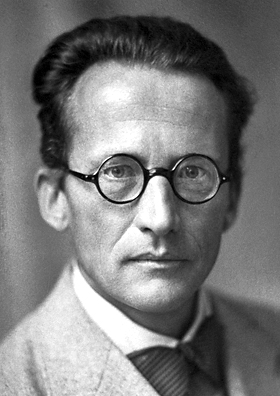
\includegraphics[width=\linewidth]{images/book4/schrodinger-1933.jpg}\par
{\footnotesize 1933 में श्रोडिंगर।}
\end{minipage}
\end{history}

\section{अभ्यास}

\begin{exercise}[$\star$]\label{exo:b3:quantum-model-systems:1}
एक इलेक्ट्रॉन (a) \qty{1.00}{nm}, (b)
\qty{0.50}{nm} लंबाई के डिब्बे में परिरुद्ध है। $E_1$ को जूल और इलेक्ट्रॉनवोल्ट में,
तथा संक्रमण $n = 1 \to 2$ का तरंगदैर्घ्य परिकलित कीजिए।
\end{exercise}

\begin{exercise}[$\star$]\label{exo:b3:quantum-model-systems:2}
घनीय \omterm{def:b3:quantum-model-systems:box}{डिब्बे में कण} के पाँच निम्नतम स्तरों को
$h^2/8mL^2$ की इकाइयों में, उनकी \omterm{def:b3:quantum-model-systems:degenerate}{अपभ्रष्टताओं} सहित, सूचीबद्ध कीजिए।
\end{exercise}

\begin{exercise}[$\star$]\label{exo:b3:quantum-model-systems:3}
\omterm{def:b3:quantum-model-systems:commutator}{क्रमविनिमेयकों} $[\hat x^2,\hat p]$ और $[\hat p^2,\hat x]$ को किसी फलन $f(x)$ पर
संक्रिया करके परिकलित कीजिए।
\end{exercise}

\begin{exercise}[$\star$]\label{exo:b3:quantum-model-systems:4}
% ledger: diat:HCl.Be
\ce{H^{35}Cl} के लिए $B = \qty{10.593}{cm^{-1}}$ लेकर स्तरों $J = 0$ से 3 की ऊर्जाएँ
(\unit{cm^{-1}} में) और \omterm{def:b3:quantum-model-systems:degenerate}{अपभ्रष्टताएँ} दीजिए, तथा अणु का जड़त्व
आघूर्ण भी।
\end{exercise}

\begin{exercise}[$\star\star$]\label{exo:b3:quantum-model-systems:5}
\omterm{def:b3:quantum-model-systems:box}{डिब्बे में कण} की अवस्था $\psi_n$ के लिए $\langle x\rangle$ और
$\langle x^2\rangle$ परिकलित कीजिए। $\langle x^2\rangle$ का मान $n = 1$ के लिए निकालिए और
उसकी तुलना चिरसम्मत मान $L^2/3$ से कीजिए, जो ऐसे कण का है जिसके कहीं भी होने की समान संभावना हो।
\end{exercise}

\begin{exercise}[$\star\star$]\label{exo:b3:quantum-model-systems:6}
% ledger: diat:H2.we, diat:D2.we
\ce{H2} और \ce{D2} की आवर्ती \omterm{def:b3:quantum-model-systems:oscillator}{शून्य-बिंदु ऊर्जाएँ}
\unit{kJ/mol} में परिकलित कीजिए, $\tilde\omega_e = \qty{4401.2}{cm^{-1}}$ और
\qty{3115.5}{cm^{-1}} से, तथा उनका अंतर भी। \omterm{def:b3:quantum-model-systems:oscillator}{समानीत द्रव्यमानों} से आप तरंग-संख्याओं के
किस अनुपात की अपेक्षा करते हैं, और मापा गया अनुपात उसके कितना निकट है?
\end{exercise}

\begin{exercise}[$\star\star$]\label{exo:b3:quantum-model-systems:7}
फलन $\phi = Nx(L - x)$ डिब्बे की मूल अवस्था का एक मोटा अनुमान है।
इसे प्रसामान्यीकृत कीजिए, फिर वास्तविक मूल अवस्था के साथ इसका अतिव्यापन
$\langle\psi_1|\phi\rangle$ परिकलित कीजिए।
\end{exercise}

\begin{exercise}[$\star\star$]\label{exo:b3:quantum-model-systems:8}
दिखाइए कि $\hat p = -\iu\hbar\,\dd/\dd x$ ऐसे फलनों के लिए \omterm{def:b3:quantum-model-systems:hermitian}{हर्मिटी} है जो
किसी अंतराल के सिरों पर लुप्त होते हैं, और कि $\hat x\hat p$ \omterm{def:b3:quantum-model-systems:hermitian}{हर्मिटी} नहीं है।
\end{exercise}

\begin{exercise}[$\star\star$]\label{exo:b3:quantum-model-systems:9}
हेक्सा-1,3,5-ट्राईन को छह $\pi$ इलेक्ट्रॉनों के रूप में मॉडल कीजिए, जो लंबाई $6l$ वाले डिब्बे में हैं, जहाँ $l =
\qty{139.7}{pm}$ (पाँच आबंध और हर सिरे पर आधा आबंध)। उसके प्रथम अवशोषण के
तरंगदैर्घ्य की भविष्यवाणी कीजिए। क्या अणु रंगीन है?
\end{exercise}

\begin{exercise}[$\star\star\star$]\label{exo:b3:quantum-model-systems:10}
चित्र के मॉडल अवरोध ($V_0 = \qty{0.40}{eV}$, $a = \qty{50}{pm}$) के लिए
$E = V_0/2$ पर, प्रोटॉन और ड्यूटेरॉन के लिए $\kappa$ परिकलित कीजिए और,
मोटे अवरोध के सूत्र से, अनुपात $T_H/T_D$। इसकी तुलना यथार्थ अनुपात, 58, से कीजिए।
\end{exercise}

\begin{exercise}[$\star\star\star$]\label{exo:b3:quantum-model-systems:11}
बेंज़ीन के छह $\pi$ इलेक्ट्रॉनों को त्रिज्या
\qty{139.7}{pm} वाले वलय पर कणों के रूप में लीजिए (C--C दूरी सम षट्भुज की त्रिज्या के बराबर है)।
स्तरों को भरिए, फिर उच्चतम भरे स्तर से निम्नतम रिक्त स्तर तक के संक्रमण का
तरंगदैर्घ्य परिकलित कीजिए।
\end{exercise}

\begin{exercise}[$\star\star\star$]\label{exo:b3:quantum-model-systems:12}
हाइड्रोजन की $1s$ अवस्था के लिए $\psi = (\pi a^3)^{-1/2}\eu^{-r/a}$। \omterm{def:b3:quantum-model-systems:hermitian}{प्रत्याशा
मान} $\langle r\rangle$ और $\langle V\rangle$ परिकलित कीजिए, और जाँचिए कि
$\langle V\rangle = 2E_1$। ($\int_0^\infty r^n\eu^{-\beta r}\dd r =
n!/\beta^{n+1}$ का उपयोग कीजिए।)
\end{exercise}

\section{समस्या: एक रंजक कितना लंबा है?}

\begin{problem}[{सप्ताहांत समस्या --- तीन सायनिन रंजकों का मुक्त-इलेक्ट्रॉन
मॉडल: केवल शृंखला क्यों विफल होती है, कौन-से संक्रमण अनुमत हैं, किसी अणु के
ऊर्जा पैमाने, और वह डिब्बा-लंबाई जो सटीक बैठती है}]
\label{pb:b3:quantum-model-systems:1}
% ledger: uvvis:cyanine, uvvis:carbocyanine, uvvis:dicarbocyanine, geo:C6H6.rCC, diat:HCl.we, diat:HCl.Be
तीन सममित सायनिन रंजक एथेनॉल में 524, 603 और 711 nm पर अवशोषण करते हैं; उनकी
संयुग्मित शृंखलाओं में, दोनों नाइट्रोजनों के बीच और उन्हें सम्मिलित करके, $j = 5$, 7
और 9 परमाणु हैं। हर आबंध $l = \qty{139.7}{pm}$ के बराबर लीजिए, $m_e =
\qty{9.109e-31}{kg}$, $h = \qty{6.626e-34}{J.s}$, $c = \qty{2.998e8}{m/s}$,
$k = \qty{1.381e-23}{J/K}$, $\qty{1}{eV} = \qty{1.602e-19}{J}$।

\medskip\noindent\textbf{भाग I --- केवल शृंखला।}
\begin{enumerate}
  \item समझाइए कि $j$ परमाणुओं की शृंखला $N = j + 1$ $\pi$ इलेक्ट्रॉन क्यों वहन करती है, और
        हर रंजक के लिए $N$ दीजिए।
  \item पहले रंजक के लिए डिब्बे के कौन-से स्तर उच्चतम भरे और निम्नतम रिक्त
        स्तर हैं?
  \item दिखाइए कि प्रथम अवशोषण $\lambda = 8mcL^2/h(N+1)$ पर है।
  \item हर शृंखला की केवल-शृंखला लंबाई $L_0 = (j - 1)l$ दीजिए।
  \item हर रंजक के लिए $\lambda$ परिकलित कीजिए, $L = L_0$ लेकर।
  \item मापे गए मानों से तुलना कीजिए। मॉडल किस दिशा में गलत है,
        और इससे $L$ के बारे में क्या पता चलता है?
\end{enumerate}

\medskip\noindent\textbf{भाग II --- कौन-से संक्रमण अनुमत हैं।}
किसी संक्रमण $n \to n'$ की तीव्रता $|\langle
\psi_n|x - L/2|\psi_{n'}\rangle|^2$ के समानुपाती है।
\begin{enumerate}[resume]
  \item दिखाइए कि $\psi_n$ डिब्बे के केंद्र के सापेक्ष सममित है, विषम
        $n$ के लिए, और प्रतिसममित, सम $n$ के लिए।
  \item निष्कर्ष निकालिए कि जब $n + n'$ सम हो तब समाकल लुप्त होता है।
  \item क्या हर रंजक का HOMO $\to$ LUMO संक्रमण अनुमत है?
  \item दूसरे रंजक के लिए, क्या HOMO से LUMO के ऊपर वाले स्तर तक का संक्रमण
        अनुमत है? और HOMO के नीचे वाले स्तर से LUMO तक का?
  \item मॉडल में, HOMO से अगला अनुमत संक्रमण किस तरंगदैर्घ्य पर (पहले वाले के
        अंश के रूप में) होगा?
  \item केवल सममिति से व्युत्पन्न ऐसा नियम मॉडल की स्थूलता के बावजूद क्यों
        बना रहता है?
\end{enumerate}

\medskip\noindent\textbf{भाग III --- किसी अणु के ऊर्जा पैमाने।}
\begin{enumerate}[resume]
  \item दूसरे रंजक के अवशोषण को eV में ऊर्जा में बदलिए।
  \item \ce{HCl} के कंपन के लिए $\tilde\omega_e = \qty{2991}{cm^{-1}}$:
        उसके क्वांटम को eV में बदलिए।
  \item \ce{HCl} के घूर्णन के लिए $B = \qty{10.59}{cm^{-1}}$: $J = 0$ और $J = 1$ के बीच के
        अंतराल को \unit{meV} में बदलिए।
  \item \qty{298}{K} पर $kT$ को \unit{meV} में परिकलित कीजिए।
  \item कक्ष ताप पर किस प्रकार के उत्तेजन समष्टित होते हैं?
  \item स्पेक्ट्रम के किन क्षेत्रों में इलेक्ट्रॉनिक, कंपनिक और
        घूर्णी संक्रमण प्रेक्षित होते हैं?
\end{enumerate}

\medskip\noindent\textbf{भाग IV --- सटीक बैठने वाला डिब्बा।}
\begin{enumerate}[resume]
  \item मापे गए 603 nm से वह लंबाई $L$ परिकलित कीजिए जो दूसरे रंजक के
        डिब्बे की होनी चाहिए।
  \item $L = L_0 + 2\delta$ लिखकर $\delta$ निकालिए।
  \item इस $\delta$ से पहले रंजक के लिए $\lambda$ की भविष्यवाणी कीजिए; आपेक्षिक
        त्रुटि दीजिए।
  \item तीसरे रंजक के लिए यही प्रश्न।
  \item $\delta$ की व्याख्या कीजिए: $\pi$ इलेक्ट्रॉन नाइट्रोजनों से आगे कहाँ
        जाते हैं?
  \item $\delta$ को आबंध-लंबाइयों में व्यक्त कीजिए, और समस्या का परिणाम
        बताइए: हर सिरे पर डिब्बे का प्रभावी विस्तार।
\end{enumerate}
\end{problem}
